\section{Introduction}

\begin{frame}
	\frametitle{Advent of AI}
	\begin{columns}
		\begin{column}{7.5cm}
			\begin{itemize}
				\item Long lasting urge to create human likenesses
				\item Used as idols in ancient religions
				\item Part of pop culture by the end of $19$th century
				\item Field of AI founded in $1956$ at Dartmouth College
				\item Researcher effusively optimistic
			\end{itemize}
		\end{column}
		\begin{column}{4cm}
			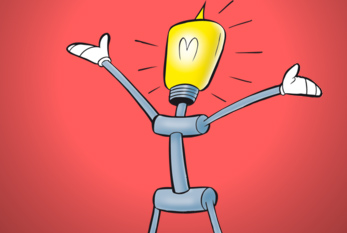
\includegraphics[width=4cm]{images/littleHelper.jpg}
		\end{column}
	\end{columns}
	\vfill
	\begin{quotation}
		``Machines will be capable, within twenty years, of doing any work a man can do.''\par\raggedleft--- \textup{Herbert Simon, 1965}
	\end{quotation}
\end{frame}

\begin{frame}
	\frametitle{Disillusionment}
	\begin{columns}
		\begin{column}{7.5cm}
			\begin{itemize}
				\item Goal too overambitious
				\item Problem broken down $\rightarrow$ task-specific solutions
				\note[item]{Perception, machine learning, planning, natural language processing etc.}
			\end{itemize}
			
			\begin{block}{Long-term goal: Machine learning}
				\begin{itemize}
					\item Learn complex behaviour
					\note[item]{perception, reasoning, intelligent control}
					\item Minimal human labour
				\end{itemize}
			\end{block}
			
			\begin{itemize}
				\item Current learning models fail, due to \emph{shallow architecture} and \emph{local estimators}
			\end{itemize}
			
		\end{column}
		\begin{column}{4cm}
			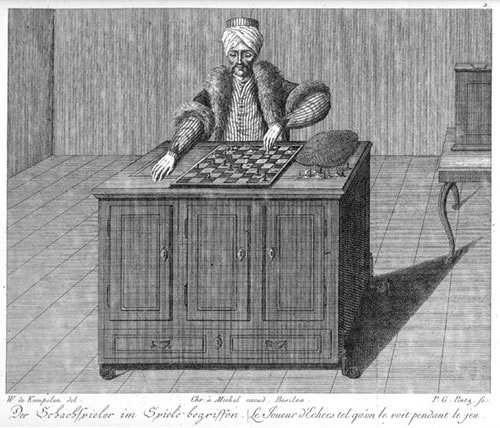
\includegraphics[width=4cm]{images/mechanical-turk.jpg}
		\end{column}
	\end{columns}
\end{frame}
